\documentclass[tikz,border=10pt]{standalone}
\usepackage{tikz}
\usepackage{amsmath}
\usetikzlibrary{shapes.geometric,arrows.meta,positioning,fit,backgrounds,shadows,decorations.pathreplacing,shapes.multipart}

\begin{document}
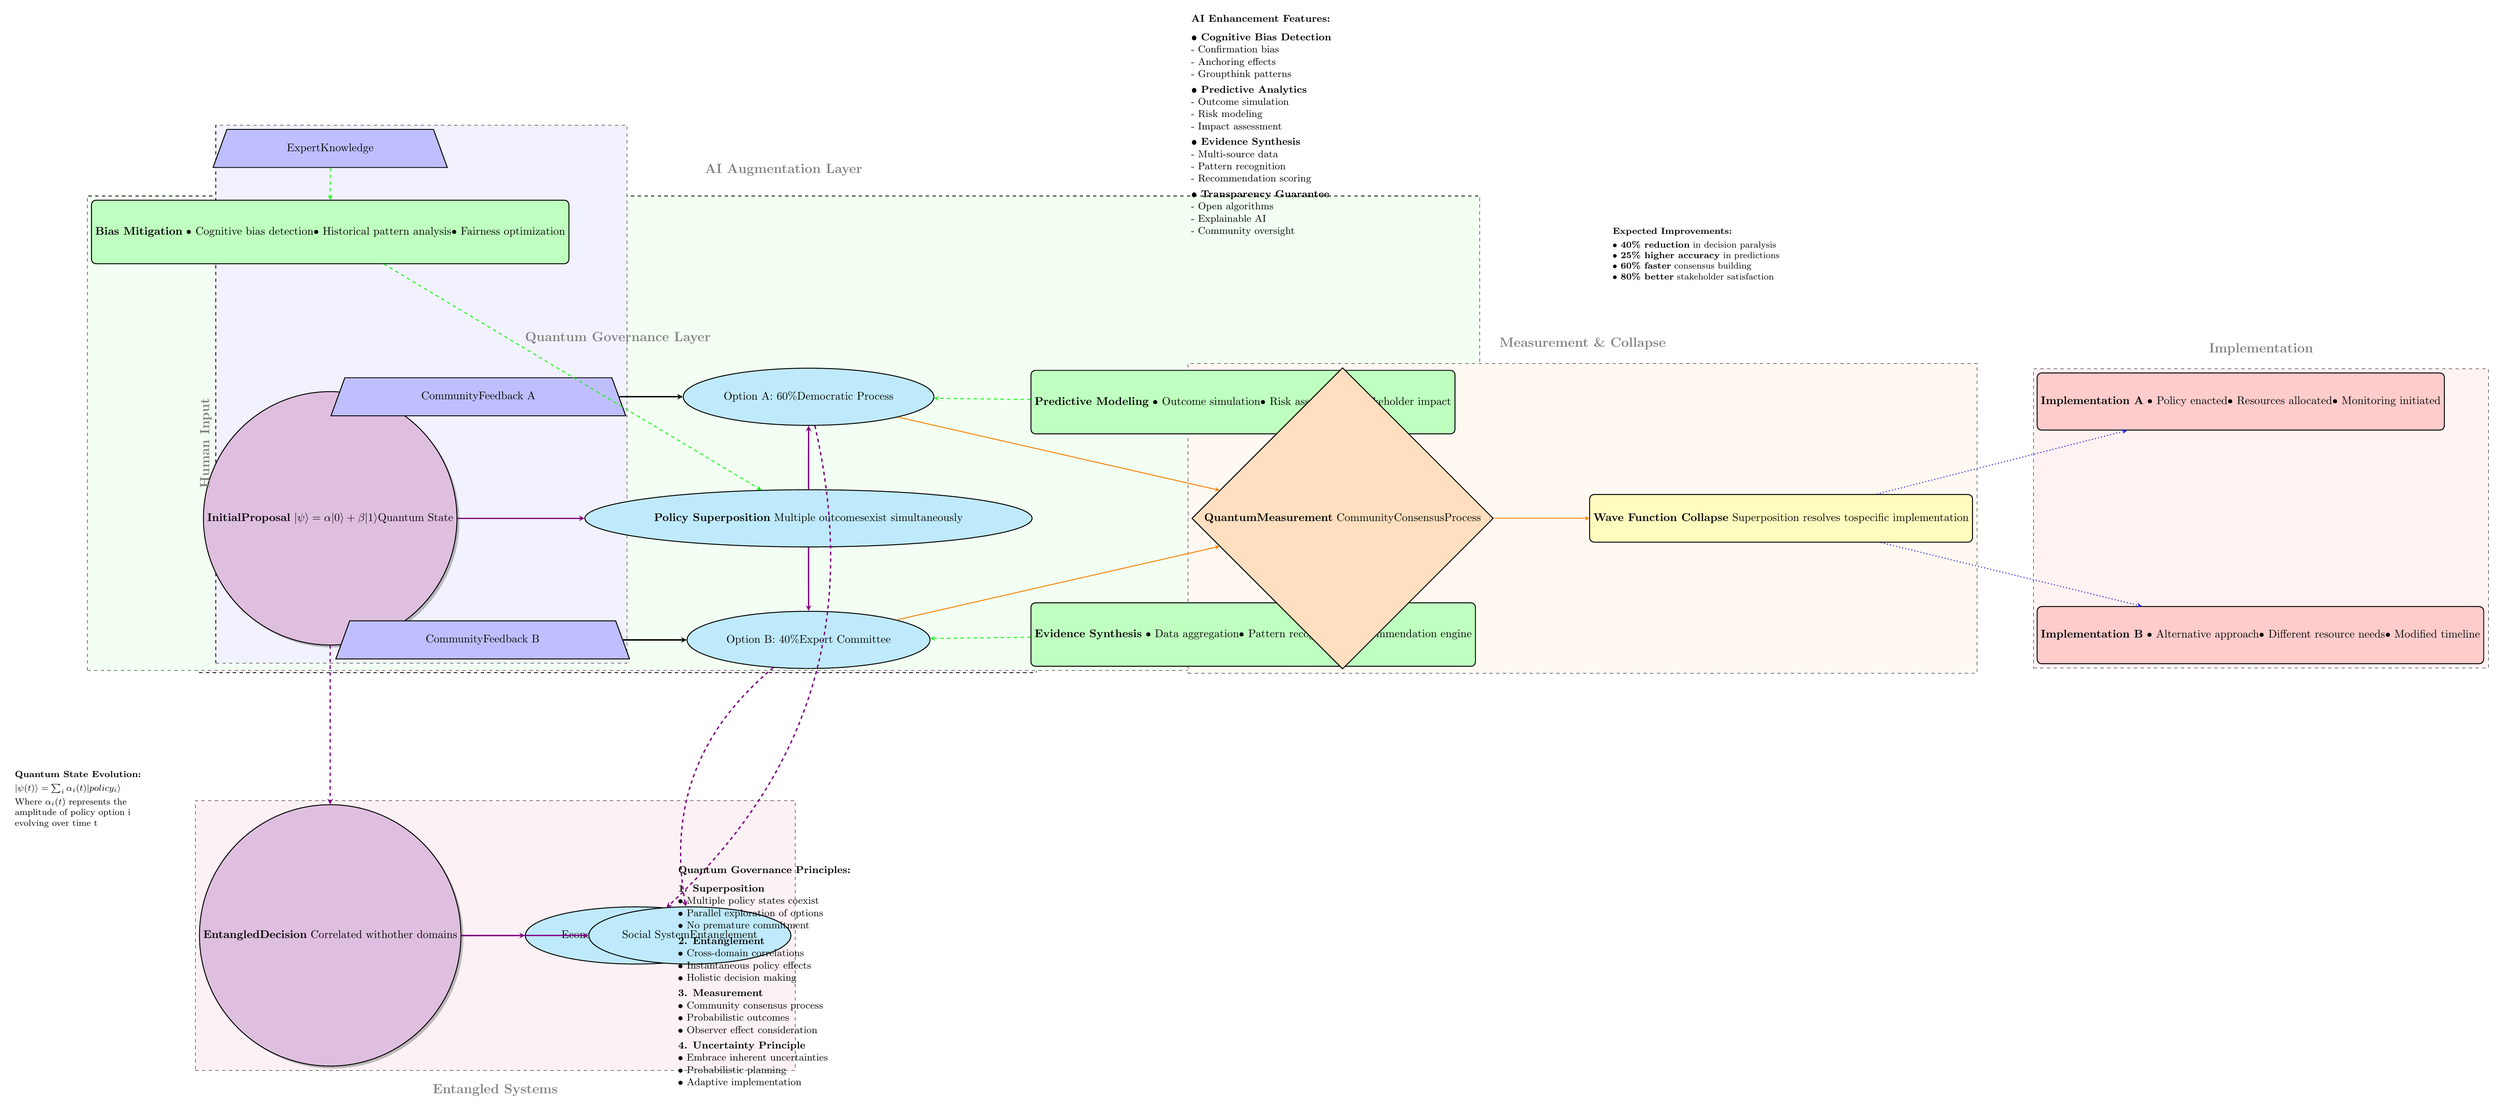
\begin{tikzpicture}[scale=1.5,
    node distance=4.5cm,
    every node/.style={font=\normalsize},
    % Quantum governance components
    quantum_state/.style={circle,draw,minimum size=2.5cm,fill=violet!25,thick,drop shadow},
    superposition/.style={ellipse,draw,minimum width=3cm,minimum height=1.8cm,fill=cyan!25,thick},
    measurement/.style={diamond,draw,minimum width=2.8cm,minimum height=2.2cm,fill=orange!25,thick},
    collapse/.style={rectangle,draw,minimum width=3.2cm,minimum height=1.5cm,fill=yellow!25,thick,rounded corners},
    ai_component/.style={rectangle,draw,minimum width=3cm,minimum height=2cm,fill=green!25,thick,rounded corners},
    human_input/.style={trapezium,trapezium left angle=70,trapezium right angle=70,draw,minimum width=2.5cm,minimum height=1.2cm,fill=blue!25,thick},
    outcome/.style={rectangle,draw,minimum width=3.5cm,minimum height=1.8cm,fill=red!20,thick,rounded corners},
    arrow/.style={->,>=stealth,very thick},
    quantum_arrow/.style={->,>=stealth,very thick,violet},
    ai_arrow/.style={->,>=stealth,thick,green,dashed},
    measurement_arrow/.style={->,>=stealth,thick,orange},
    probability/.style={->,>=stealth,thick,blue,dotted}
]

% Initial Proposal State
\node[quantum_state] (initial_proposal) {
    \textbf{Initial}\\
    \textbf{Proposal}\\[0.2cm]
    $|\psi\rangle = \alpha|0\rangle + \beta|1\rangle$\\
    Quantum State
};

% Superposition Phase
\node[superposition,right=4cm of initial_proposal] (policy_superposition) {
    \textbf{Policy Superposition}\\[0.1cm]
    Multiple outcomes\\
    exist simultaneously
};

\node[superposition,above=2cm of policy_superposition] (option_a) {
    Option A: 60\%\\
    Democratic Process
};

\node[superposition,below=2cm of policy_superposition] (option_b) {
    Option B: 40\%\\
    Expert Committee
};

% AI Augmentation Layer
\node[ai_component,above=4cm of initial_proposal] (bias_mitigation) {
    \textbf{Bias Mitigation}\\[0.1cm]
    • Cognitive bias detection\\
    • Historical pattern analysis\\
    • Fairness optimization
};

\node[ai_component,above right=2cm and 2cm of policy_superposition] (impact_modeling) {
    \textbf{Predictive Modeling}\\[0.1cm]
    • Outcome simulation\\
    • Risk assessment\\
    • Stakeholder impact
};

\node[ai_component,below right=2cm and 2cm of policy_superposition] (evidence_synthesis) {
    \textbf{Evidence Synthesis}\\[0.1cm]
    • Data aggregation\\
    • Pattern recognition\\
    • Recommendation engine
};

% Human Input Components
\node[human_input,left=2cm of option_a] (community_input_a) {
    Community\\
    Feedback A
};

\node[human_input,left=2cm of option_b] (community_input_b) {
    Community\\
    Feedback B
};

\node[human_input,above=1cm of bias_mitigation] (expert_input) {
    Expert\\
    Knowledge
};

% Measurement/Observation Phase
\node[measurement,right=5cm of policy_superposition] (quantum_measurement) {
    \textbf{Quantum}\\
    \textbf{Measurement}\\[0.2cm]
    Community\\
    Consensus\\
    Process
};

% State Collapse
\node[collapse,right=3cm of quantum_measurement] (state_collapse) {
    \textbf{Wave Function Collapse}\\[0.1cm]
    Superposition resolves to\\
    specific implementation
};

% Final Outcomes
\node[outcome,above right=2cm and 2cm of state_collapse] (outcome_a) {
    \textbf{Implementation A}\\[0.1cm]
    • Policy enacted\\
    • Resources allocated\\
    • Monitoring initiated
};

\node[outcome,below right=2cm and 2cm of state_collapse] (outcome_b) {
    \textbf{Implementation B}\\[0.1cm]
    • Alternative approach\\
    • Different resource needs\\
    • Modified timeline
};

% Entanglement Network
\node[quantum_state,below=5cm of initial_proposal] (entangled_decision) {
    \textbf{Entangled}\\
    \textbf{Decision}\\[0.2cm]
    Correlated with\\
    other domains
};

\node[superposition,right=2cm of entangled_decision] (economic_entanglement) {
    Economic Policy\\
    Entanglement
};

\node[superposition,right=4cm of entangled_decision] (social_entanglement) {
    Social System\\
    Entanglement
};

% Background groupings
\begin{scope}[on background layer]
\node[fill=violet!5,draw,dashed,fit=(initial_proposal)(policy_superposition)(option_a)(option_b)] (quantum_layer) {};
\node[fill=green!5,draw,dashed,fit=(bias_mitigation)(impact_modeling)(evidence_synthesis)] (ai_layer) {};
\node[fill=blue!5,draw,dashed,fit=(community_input_a)(community_input_b)(expert_input)] (human_layer) {};
\node[fill=orange!5,draw,dashed,fit=(quantum_measurement)(state_collapse)] (measurement_layer) {};
\node[fill=red!5,draw,dashed,fit=(outcome_a)(outcome_b)] (outcome_layer) {};
\node[fill=purple!5,draw,dashed,fit=(entangled_decision)(economic_entanglement)(social_entanglement)] (entanglement_layer) {};
\end{scope}

% Quantum Evolution
\draw[quantum_arrow] (initial_proposal) -- (policy_superposition);
\draw[quantum_arrow] (policy_superposition) -- (option_a);
\draw[quantum_arrow] (policy_superposition) -- (option_b);

% AI Integration
\draw[ai_arrow] (bias_mitigation) -- (policy_superposition);
\draw[ai_arrow] (impact_modeling) -- (option_a);
\draw[ai_arrow] (evidence_synthesis) -- (option_b);
\draw[ai_arrow] (expert_input) -- (bias_mitigation);

% Human Input
\draw[arrow] (community_input_a) -- (option_a);
\draw[arrow] (community_input_b) -- (option_b);

% Measurement Process
\draw[measurement_arrow] (option_a) -- (quantum_measurement);
\draw[measurement_arrow] (option_b) -- (quantum_measurement);
\draw[measurement_arrow] (quantum_measurement) -- (state_collapse);

% Outcome Probabilities
\draw[probability] (state_collapse) -- (outcome_a);
\draw[probability] (state_collapse) -- (outcome_b);

% Entanglement Relations
\draw[quantum_arrow,dashed] (initial_proposal) -- (entangled_decision);
\draw[quantum_arrow] (entangled_decision) -- (economic_entanglement);
\draw[quantum_arrow] (entangled_decision) -- (social_entanglement);

% Cross-entanglement effects
\draw[quantum_arrow,bend left=30,dashed] (option_a) to (economic_entanglement);
\draw[quantum_arrow,bend right=30,dashed] (option_b) to (social_entanglement);

% Labels
\node[above=0.5cm of quantum_layer,font=\large,text=gray] {\textbf{Quantum Governance Layer}};
\node[above=0.5cm of ai_layer,font=\large,text=gray] {\textbf{AI Augmentation Layer}};
\node[left=0.3cm of human_layer,font=\large,text=gray,rotate=90] {\textbf{Human Input}};
\node[above=0.3cm of measurement_layer,font=\large,text=gray] {\textbf{Measurement \& Collapse}};
\node[above=0.3cm of outcome_layer,font=\large,text=gray] {\textbf{Implementation}};
\node[below=0.3cm of entanglement_layer,font=\large,text=gray] {\textbf{Entangled Systems}};

% Quantum Principles Box
\node[below right=8cm and 8cm of initial_proposal,font=\small,align=left] (principles) {
    \textbf{Quantum Governance Principles:}\\[0.2cm]
    \textbf{1. Superposition}\\
    • Multiple policy states coexist\\
    • Parallel exploration of options\\
    • No premature commitment\\[0.1cm]
    \textbf{2. Entanglement}\\
    • Cross-domain correlations\\
    • Instantaneous policy effects\\
    • Holistic decision making\\[0.1cm]
    \textbf{3. Measurement}\\
    • Community consensus process\\
    • Probabilistic outcomes\\
    • Observer effect consideration\\[0.1cm]
    \textbf{4. Uncertainty Principle}\\
    • Embrace inherent uncertainties\\
    • Probabilistic planning\\
    • Adaptive implementation
};

% AI Enhancement Box
\node[above left=8cm and 8cm of state_collapse,font=\small,align=left] (ai_enhancement) {
    \textbf{AI Enhancement Features:}\\[0.2cm]
    \textbf{• Cognitive Bias Detection}\\
    - Confirmation bias\\
    - Anchoring effects\\
    - Groupthink patterns\\[0.1cm]
    \textbf{• Predictive Analytics}\\
    - Outcome simulation\\
    - Risk modeling\\
    - Impact assessment\\[0.1cm]
    \textbf{• Evidence Synthesis}\\
    - Multi-source data\\
    - Pattern recognition\\
    - Recommendation scoring\\[0.1cm]
    \textbf{• Transparency Guarantee}\\
    - Open algorithms\\
    - Explainable AI\\
    - Community oversight
};

% Quantum Mathematics Annotation
\node[below left=5cm and 3cm of initial_proposal,font=\footnotesize,align=left] (quantum_math) {
    \textbf{Quantum State Evolution:}\\[0.1cm]
    $|\psi(t)\rangle = \sum_i \alpha_i(t)|policy_i\rangle$\\[0.1cm]
    Where $\alpha_i(t)$ represents the\\
    amplitude of policy option i\\
    evolving over time t
};

% Performance Metrics
\node[above right=5cm and 6cm of quantum_measurement,font=\footnotesize,align=left] (metrics) {
    \textbf{Expected Improvements:}\\[0.1cm]
    • \textbf{40\% reduction} in decision paralysis\\
    • \textbf{25\% higher accuracy} in predictions\\
    • \textbf{60\% faster} consensus building\\
    • \textbf{80\% better} stakeholder satisfaction
};

\end{tikzpicture}
\end{document}
